\documentclass[12t,letterpaper]{article}

\newenvironment{proof}{\noindent{\bf Proof:}}{\qed\bigskip}

\newtheorem{theorem}{Theorem}
\newtheorem{corollary}{Corollary}
\newtheorem{lemma}{Lemma} 
\newtheorem{claim}{Claim}
\newtheorem{fact}{Fact}
\newtheorem{definition}{Definition}
\newtheorem{assumption}{Assumption}
\newtheorem{observation}{Observation}
\newtheorem{example}{Example}
\newcommand{\qed}{\rule{7pt}{7pt}}

\newcommand{\assignment}[4]{
\thispagestyle{plain} 
\newpage
\setcounter{page}{1}
\noindent
\begin{center}
\framebox{ \vbox{ \hbox to 6.28in
{\bf CS 194: Parallel Computing \hfill #1}
\vspace{4mm}
\hbox to 6.28in
{\hspace{2.5in}\large\mbox{#2}}
\vspace{4mm}
\hbox to 6.28in
{{\it Handed Out: #3 \hfill Due: #4}}
}}
\end{center}
}

\newcommand{\solution}[3]{
\thispagestyle{plain} 
\newpage
\setcounter{page}{1}
\noindent
\begin{center}
\framebox{ \vbox{ \hbox to 6.28in
{\bf CS 194 \hfill #3}
\vspace{4mm}
\hbox to 6.28in
{\hspace{2.5in}\large\mbox{#2}}
\vspace{4mm}
\hbox to 6.28in
{#1 \hfill}
}}
\end{center}
\markright{#1}
}

\newenvironment{algorithm}
{\begin{center}
\begin{tabular}{|l|}
\hline
\begin{minipage}{1in}
\begin{tabbing}
\quad\=\qquad\=\qquad\=\qquad\=\qquad\=\qquad\=\qquad\=\kill}
{\end{tabbing}
\end{minipage} \\
\hline
\end{tabular}
\end{center}}

\def\Comment#1{\textsf{\textsl{$\langle\!\langle$#1\/$\rangle\!\rangle$}}}


\usepackage{amsmath, dsfont, hyperref, xcolor}

\oddsidemargin 0in
\evensidemargin 0in
\textwidth 6.5in
\topmargin -0.5in
\textheight 9.0in
\newcommand{\norm}[1]{\left\lVert #1 \right\rVert}
\newcommand{\?}{\stackrel{?}{=}}

\usepackage{graphicx}

\begin{document}

\solution{Harry He, Kada Situ, Brian SungYong Park, Conrad Yuan Shiao, Nikhil Unni}{Baseline for Class Project}{Fall 2015}
\pagestyle{myheadings}
\section{Project Description}
    The goal of this project is to optimize PIGZ, which is a parallel version of GZIP, a popular compression software in UNIX. PIGZ has already been parallelized using Pthreads in CPU and has achieved a linear speedup. However, with the rise of general purpose GPUs, we believe there is an opportunity to improve upon the PIGZ implementation. Our plan is to use CUDA technology to make use of the GPU to attempt to achieve further performance speedup during different stages of the compression algorithm, all the while trying to not significantly sacrifice the compression ratio. Because pigz uses zlib as its compression library, a large portion of our project will be making major changes in the zlib folder to use the GPU.

\section{Code Description}
Github Repository: \url{https://github.com/CS194-project/CS194-project}\\
Testing Data Website: \url{http://sun.aei.polsl.pl/~sdeor/index.php?page=silesia}\\

The ``pigz'' and ``zlib'' directories make up functional part of the project. The corpus directory stores the benchmark testing data. Other directories contain mainly reference code.
Run ``make'' under root directory to build pigz and zlib. Inside pigz directory, ``pigz'' is parallelized version of pigz and ``pignz'' is the single threaded version of pigz. 

\section{Testing Data Description}
We use Silesia Corpus as our testing data set. The corpus includes files with different formats in various sizes (ranging from 6MB to 51MB), which is great for testing compression efficiency. The actual data is not included in the repository. Run “make corpus” to download the testing data. Inside corpus folder, ``.orig'' files are the files downloaded. ``.big'' files are big data which are the combination of 10 copies of corresponding .orig files. ``combined'' file is the combination of all ``.orig'' files. Our benchmarking is based on all ``.big'' files and the ``combined'' file.

\section{Steps to Run Benchmark Code}
\begin{enumerate}
  \item Clone the repository\\
    {\color{blue}\$ git clone https://github.com/CS194-project/CS194-project.git}\\
    If you want a more verbose benchmarking output, change to ``benchmark'' branch. ({\color{blue}\$ git checkout benchmark})
  \item Download Silesia corpus benchmark files\\
    {\color{blue}\$ make corpus}\\
  \item Build pigz (both serial/parallel) and zlib\\
    {\color{blue}\$ make}\\    
  \item Run benchmark\\
    {\color{blue}\$ make benchmark}\\
\end{enumerate}
\section{Testing Machine}

\begin{itemize}
\item Machine IP: hive1.cs.berkeley.edu
\item Memory size: 32GB
\item CPU: Intel(R) Core(TM) i7-4770 CPU @ 3.40GHz
\item Number of cores: 4
\item Number of hardware threads: 8
\item L1 instruction cache: 32KB, 8-way, 64B cache line
\item L1 data cache: 32KB, 8-way, 64B cache line
\item L2 cache: 256KB, 8-way, 64B cache line
\item L3 cache: 8MB, 16-way, 64B cache line
\item Max memory bandwidth: 25.6 GB/s
\item Supported SIMD instruction: SSE 4.1/4.2
\item GPU: Geforce GT 740
\item GPU Memory Size: 1GB
\item Base clock: 993 MHz
\item Number of CUDA cores: 384
\item GPU Memory Bandwidth: 80 GB/s
\item CUDA Compute Capability: 3.0
\item CUDA library version: 7.5
\end{itemize}

\section{Benchmark}
Running the serial version on our corpus we get:\\
\begin{center}
\begin{tabular}{ |c|c|c|c|c|c|c| } 
 \hline
 Corpus & Total Time (s) & IO Time (s) & Speed (MB/s) & Input Size (byte) & Output Size (byte) & Compression Ratio\\
 \hline
combine & 7.045 & 0.046 & 28.878 & 211938890 & 78351541 & 2.705\\
\hline
dickens & 3.928 & 0.025 & 24.899 & 10192446 & 4725440 & 2.157\\
\hline
mozilla & 1.823 & 0.012 & 26.967 & 51220480 & 20783147 & 2.465\\
\hline
mr & 0.343 & 0.002 & 27.942 & 9970564 & 3886965 & 2.565\\
\hline
nci & 0.707 & 0.006 & 45.627 & 33553445 & 4500144 & 7.456\\
\hline
ooffice & 0.271 & 0.002 & 21.806 & 6152192 & 3343141 & 1.84\\
\hline
osdb & 0.362 & 0.002 & 26.711 & 10085684 & 4138273 & 2.437\\
\hline
reymont & 0.226 & 0.001 & 28.175 & 6627202 & 2386691 & 2.777\\
\hline
samba & 0.623 & 0.004 & 33.326 & 21606400 & 6216311 & 3.476\\
\hline
sao & 0.374 & 0.002 & 18.604 & 7251944 & 5670905 & 1.279\\
\hline
webster & 1.434 & 0.009 & 27.739 & 41458703 & 15334578 & 2.704\\
\hline
xml & 0.145 & 0.001 & 35.511 & 5345280 & 1148727 & 4.653\\
\hline
x-ray & 0.417 & 0.003 & 19.5 & 8474240 & 6205547 & 1.366\\
\hline
\end{tabular}
1. Serial Baseline
\end{center}

And running the full parallel version of pigz on the corpus we get:\\

\begin{center}
\begin{tabular}{ |c|c|c|c|c|c|c| } 
 \hline
Corpus & Total Time (s) & IO Time (s) & Speed (MB/s) & Input Size (byte) & Output Size (byte) & Compression Ratio\\
\hline
combine & 5.287 & 4.568 & 281.313 & 211938890 & 78351541 & 2.705\\
\hline
dickens & 0.249 & 0.196 & 180.796 & 10192446 & 4725440 & 2.157\\
\hline
mozilla & 1.380 & 1.162 & 223.733 & 51220480 & 20783147 & 2.465\\
\hline
mr & 0.227 & 0.186 & 231.616 & 9970564 & 3886965 & 2.565\\
\hline
nci & 0.818 & 0.768 & 632.326 & 33553445 & 4500144 & 7.456\\
\hline
oofice & 0.159 & 0.121 & 156.694 & 6152192 & 3343141 & 1.840\\
\hline
osdb & 0.173 & 0.113 & 161.243 & 10085684 & 4138273 & 2.437\\
\hline
reymont & 0.166 & 0.130 & 179.688 & 6627202 & 2386691 & 2.777\\
\hline
samba & 0.449 & 0.367 & 249.627 & 21606400 & 6216311 & 3.476\\
\hline
sao & 0.198 & 0.137 & 112.528 & 7251944 & 5670905 & 1.279\\
\hline
webster & 1.121 & 0.967 & 257.036 & 41458703 & 15334578 & 2.704\\
\hline
xml & 0.098 & 0.073 & 197.823 & 5345280 & 1148727 & 4.653\\
\hline
x-ray & 0.174 & 0.101 & 110.974 & 8474240 & 6205547 & 1.366\\
\hline
\end{tabular}
2. Full Parallel Baseline
\end{center}

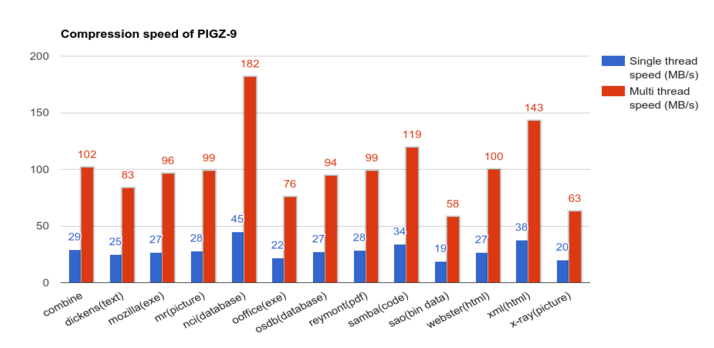
\includegraphics[width=1\textwidth]{screen1}
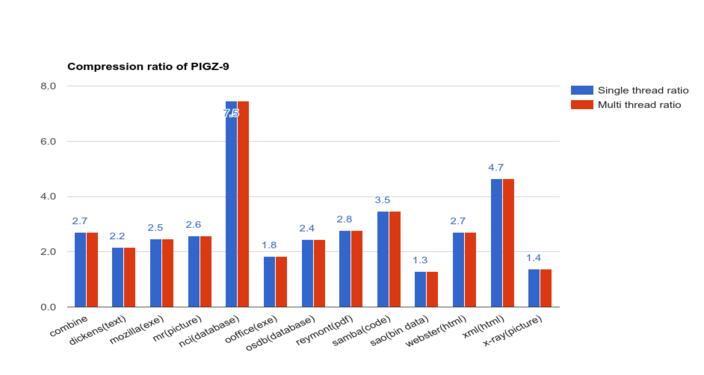
\includegraphics[width=1\textwidth]{screen2}

\section{Appendix : PIGZ Profiling}
We used the Linux “perf” tool to determine the time consumption of each functions.

Command under pigz folder:\\
{\color{blue} \$ sudo perf record ./pigz -k -9 corpus/combined}\\
{\color{blue} \$ sudo perf report}\\

\end{document}
